% !TeX root=../../main.tex

\chapter{شبکه‌های عصبی کانلوشنی}
\label{appex:cnn}

شبکه‌های عصبی مصنوعی مدل‌هایی هستند که در بسیاری از زمینه‌های تحقیقاتی از جمله یادگیری ماشین کاربرد دارند. یک شبکه عصبی مصنوعی از واحدهای ساده ای به نام \gls{neuron} تشکیل شده است که در یک سیستم پیچیده سازمان یافته اند. هر \gls{neuron} بر اساس ورودی‌های خود، یک خروجی (\gls{activation}‌) را محاسبه می‌کند که می‌تواند فعالیت‌ها یا داده‌های سایر \glspl{neuron} باشد. متداول‌ترین نوع شبکه عصبی،  شبکه عصبی کاملاً متصل \gls{fullyconnectedffnn} است. این شبکه‌ها دارای ورودی (جایی که داده‌ها وارد می‌شوند) و خروجی‌ هستند. به طور معمول، هدف از استفاده از این مدل‌ها حل \gls{regression} یا \gls{classification}، توسط تقریب \gls{activation} خروجی با مقدار هدف، برای هر داده ورودی است. این شبکه‌ها به صورت \glspl{layer} متوالی سازماندهی شده اند که یک \gls{neuron}(واحد) از لایه $k$ تمام \glspl{neuron} \gls{layer} $k-1$ را به عنوان ورودی دریافت می‌کند، ترکیبی خطی از این مقادیر را محاسبه کرده و آن را از طریق تابع غیر خطی عبور می‌دهد

محاسبه خروجی
\gls{neuron} \lr{i}ام \gls{layer} \lr{k}
\begin{equation}
	O_{k, i}=\operatorname{actv}\left(\mathrm{W}_{k, \mathrm{i}} \cdot \mathrm{l}_{\mathrm{k}-1}+b_{k, i}\right)
	\label{eq:ch_lr:activation_out}
\end{equation}

که $O_{k,i}$ واحد $i$ام \gls{layer} $k$  و $l_{k-1}$ بردار تمام \glspl{activation}ی \gls{layer} $k-1$ است. بردار $W_{k,i}$ و عدد $b_{k,i}$ پارامترهای ما هستند که اغلب به آنها \gls{netweight} گفته می‌شود که برای یک وظیفه خاص آموخته می‌شوند. تابع \gls{activation} غیرخطی \lr{actv} می‌تواند اشکال مختلفی  به خود بگیرد. هر مدل با یک لایه پنهان و تعداد مشخصی نورون اگر پارامترهای کافی داشته باشد می‌تواند هر تابع پیوسته ای را با خطا دلخواه تقریب بزند\cite{dhungel2017fully}.


\glspl{convnet}  یک نوع شبکه عصبی مصنوعی هستند که از نورون‌ها، لایه‌ها و وزن‌ها تشکیل شده اند. مطالعه ای که در سال 1968 میلادی صورت گرفت نشان داد که قشر بینایی مغز برای پردازش اطلاعات از تصاویر از الگوی پیچیده ای استفاده می‌نماید\cite{sutherland1968outlines}. نواحی ادراکی که قشر بینایی در آن قرار دارد، همانند فیلترهای محلی بر روی اطلاعات تصویر اعمال می‌شود. سلول‌های ساده‌تر برای تشخیص ویژگی‌های ادراکی سطح پایین‌تر در نواحی ادراکی مانند لبه‌ها کاربرد دارند، همچنین سلول‌های پیچیده قادر به تشخیص ویژگی‌های مهم‌تر و اختصاصی‌تر و در سطوح بالاتر می‌باشند. تشخیص ویژگی‌های اختصاصی‌تر نتیجه و ترکیبی از ویژگی‌های سطح پایین می‌باشد. این عملکرد مغز الهام بخش شبکه‌های عصبی عمیق امروزی می‌باشد. مفهوم شبکه کانولوشن نخستین بار در سال 1980 توسط فکوشیما مطرح گردید\cite{fukushima2007neocognitron}. اما به دلیل نیاز به سخت افزار ها و پردازشگر‌های گرافیکی قوی استفاده از این شبکه ها برای تشخیص تا سال 2012 که به شکل اختصاصی برای تشخیص تصاویر ارایه و معرفی گریدی به تعویق افتاد\cite{lecun2015deep}.

\begin{figure}[!ht]
	\centerline{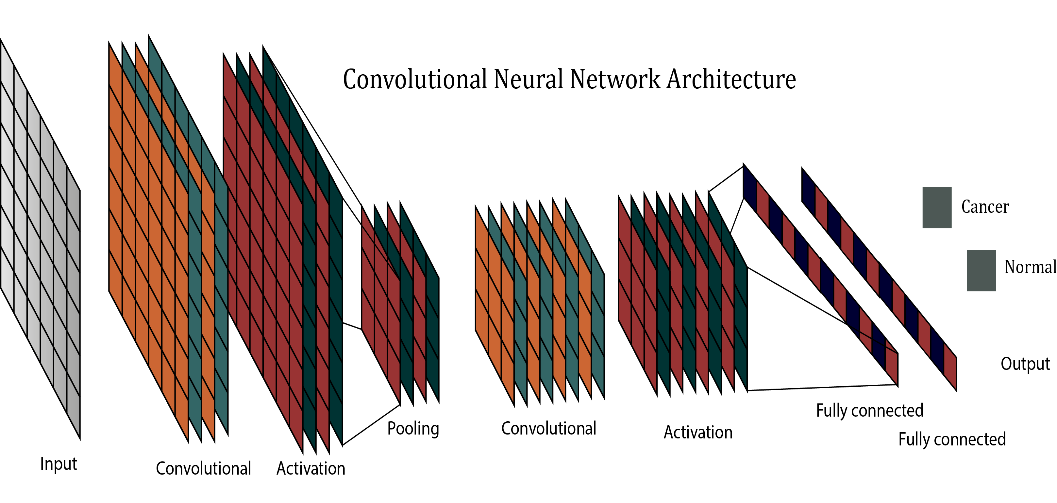
\includegraphics[width=14cm]{chaps/lr/cnn_arch}}
	\caption{معماری یک شبکه عصبی کانولوشنی}
	\label{fig:ch_lr:cnn_arch}
\end{figure}

همانطور که قبلاً بیان شد، \glspl{convnet} مدل‌های \gls{fullyconnectedffnn} هستند که از لایه‌های زیادی تشکیل شده اند. بسیاری از این مدل‌ها محدودیت‌های پارامتر و مکانی دارند که در ادامه توضیح داده خواهد شد. با این حال، آنها در تغییراتی که بر ورودی‌شان اعمال می‌کنند تفاوت دارند. در اینجا ما تمام لایه‌های یک شبکه کانولوشنی و توابع مورد استفاده در آموزش آن‌ها را شرح می‌دهیم. یک معماری می‌تواند یاد بگیرد که مسائل بسیار متفاوتی را حل کند تا زمانی که پارامترها برای هر یک از مسائل به خوبی بهینه شوند.

لایه ورودی فقط نمایشی از داده خام است که به مدل داده می‌شود که نیاز به شکل ورودی ثابت دارد. در رایج ترین حالت، یک تصویر به یک آرایه 3 \gls{dimension}ی تبدیل می‌شود با ابعاد [$w, h,3$] که $w$ و $h$ عرض و ارتفاع هستند. \gls{dimension} آخر به دلیل استفاده از تصاویر رنگی \lr{RGB\LTRfootnote{Red Green Blue}} اغلب $3$ است. وقتی از تصاویر \gls{xray} استفاده می‌کنیم چون دارای یک \gls{channel} \gls{intensity} هستند \gls{dimension} سوم برابر با $1$ است.

این لایه اصلی ترین لایه شبکه‌های عصبی کانولوشنی است و این شبکه‌ها نام‌ خود را از این لایه‌ها دریافت می‌کنند. وظیفه این لایه استخراج ویژگی‌ها است. این لایه عملیات کانولوشن را بر روی داده ورودی اعمال می‌کند و خروجی‌هایی به نام \gls{featuremap} از این لایه به دست می‌آید. در نتیجه تمامی نورون‌ها در یک \gls{featuremap}، وزن‌ها و \glspl{bias} مشابه و مشترکی دارند که باعث می‌شود، ویژگی‌های تصویر در موقعیت‌های مختلف قابل شناسایی باشند. از طرف دیگر این اشتراک وزن‌ها باعث کاهش تعداد پارامتر‌های مورد نیاز برای آموزش می‌شود. در شبکه‌های کانولوشن اتصالات به صورت نواحی کوچک و محلی صورت می‌گیرد. به بیان دیگر هر نورون در نخستین لایه مخفی به ناحیه کوچکی از نورون‌های ورودی متصل می‌شود. برای مثال اگر این ناحیه $5\times 5$ باشد این ناحیه کوچک $25$ پیکسلی \gls{localreceptivefield}  یا \gls{kernel} کانولوشن نامیده می‌شود. با توجه به شکل \ref{fig:ch_lr:cnn_conv5} یک تصویر ورودی $28\times 28$ داریم که یک \gls{kernel} $5\times 5$ بر روی پیکسل‌های ورودی از چپ به راست حرکت می‌کند هر پنجره به نورونی در لایه مخفی متصل می‌شود. بناباین همان طور که در شکل \ref{fig:ch_lr:cnn_conv5} مشخص است لایه مخفی شامل یک شبکه $24\times 24$ نورونی خواهد بود.

\begin{figure}[!ht]
	\centerline{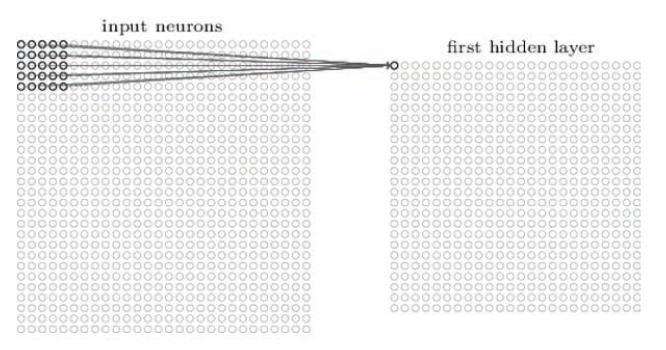
\includegraphics[width=11cm]{chaps/lr/cnn_conv5}}
	\caption{
		عملیات \gls{convolution} در یک \gls{convnet} با \gls{kernel} $5\times 5$
	}
	\label{fig:ch_lr:cnn_conv5}
\end{figure}

در شکل \ref{fig:ch_lr:cnn_conv5} هر نورون لایه مخفی دارای یک \gls{bias} و تعداد $5\times 5$ وزن می‌باشد که به  ناحیه ادراکی خود متصل شده است. تمامی نورون‌های لایه مخفی مذکور که دارای ابعاد $24\times 24$ هستند، دارای وزن‌ها و \glspl{bias}ی مشترکی می‌باشند. به عبارت دیگر خروجی نورون لایه کانولوشن $y_{w,h,m}$ در طول و عرض $w,h$ و عمق $m$ به صورت رابطه \ref{eq:ch_lr:neuron_ouput} است.
\begin{equation}
	y_{w,h,m} = f\left(\sum_{i=(w-1)S+1}^{(w-1)S+K} \sum_{j=(h-1)S+1}^{(h-1)S+K} \sum_{k=1}^{N} W_{k,m}(x_{i,j,k})+b_m\right)
	\label{eq:ch_lr:neuron_ouput}
	%	\caption{خروجی نورون لایه کانولوشن}
\end{equation}

که در این رابطه $f$ \gls{activationfunction}، $b_m$ بایاس مشترک نورون‌ها، $W_{k,m}$ وز‌ن‌های $5\times 5$ مشترک نورون‌ها و $x_{i,j,k}$ ورودی در موقعیت $i,j,k$ می‌باشد. بنابراین تمامی نورون‌های واقع در لایه مخفی اول به طور دقیق ویژگی‌های مشابهی را در نواحی مختلف تصویر شناسایی می‌کنند. در نهایت خروجی لایه ورودی یا نورون‌های لایه مخفی به عنوان \gls{featuremap} شناخته می‌شوند. ابعاد مربوط به ماتریس خروجی لایه کانولوشن $W_2\times H_2 \times D_2$ که از ماتریس ورودی با ابعاد $W_1\times H_1 \times D_1$ است، به صورت رابطه \ref{eq:ch_lr:conv_ouput} به دست می‌آید.

\begin{equation}
	W_2 = \frac{W_1-F+2P}{S+1}, \qquad H_2=\frac{H_1-F+2P}{S+1}, \qquad D_2=K
	\label{eq:ch_lr:conv_ouput}
\end{equation}
در روابط \ref{eq:ch_lr:conv_ouput} که بیانگر نحوه محاسبه ابعاد ماتریس خروجی کانولوشن است،
$F, P, S$ و $k$
به ترتیب نشان دهنده اندازه \gls{kernel}، مدار \gls{zeropadding}، اندازه \gls{stride} و تعداد فیلترها می‌باشد. طبق این روابط به ازای هر فیلتر تعداد $F\times F\times D_1$ وزن داریم و با توجه به تعداد $k$ فیلتر موجود، در مجموع تعداد $k(F\times F\times D_1)$ وزن و $k$ بایاس ایجاد می‌شود. بنابراین تعداد پارامترهایی که شبکه در یک لایه کانولوشن خود می‌بایست آموزش ببیند زیاد است.

بکارگیری \gls{activationfunction} در لایه کانولوشن باعث ایجاد خصوصیات غیر خطی در خروجی می‌شود و باعث می‌شود عملکرد مدل متمایز کننده‌تر شود. این توابع با حفظ اندازه لایه، بدون نیاز به پارامترهای آموخته شده، یک عملكرد ساده عنصرگونه در مدل انجام می‌دهند. تابع \gls{relu} متداول ترین تابع مورد استفاده به خاطر آسان کردن مرحله آموزش است. مثال‌های دیگر شامل تابع \gls{sigmoid} و \gls{hyperbolictangent} است.
\begin{equation}
	\begin{aligned}
		\text{ReLU:}&\quad r_{m,n,c} = \max\{0,l_{x,y,z}\} \\
		\text{Sigmoid:}&\quad s_{m,n,c} = \frac{1}{1-\exp(-l_{x,y,z})}
	\end{aligned}
	\label{eq:ch_lr:relu-sigmoid}
\end{equation}
\begin{figure}[!ht]
	\centerline{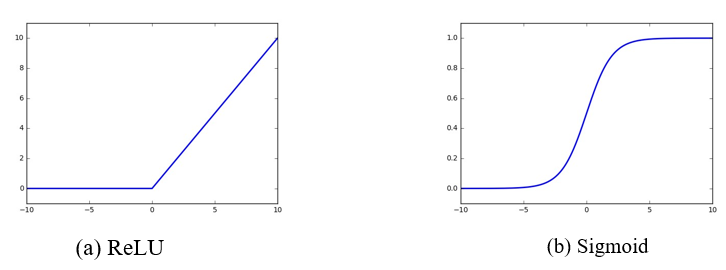
\includegraphics[width=14cm]{chaps/lr/activation_functions}}
	\caption{(\lr{a}) \gls{activationfunction} \lr{ReLU} و (\lr{b}) \gls{activationfunction} \gls{sigmoid}	
	}
	\label{fig:ch_lr:activation_functions}
\end{figure}
در یک شبکه عصبی کانولوشن معمولا پس از هر لایه کانولوشن یک لایه \lr{pooling} قرار می‌گیرد . این لایه‌ از آن جهت اهمیت دارد که باعث کاهش تعداد پارامترهایی می‌شود که باید آموزش ببینند. بنابراین با بکارگیری این لایه ضمن کاهش محاسبات مورد نیاز در بخش آموزش، باعث کنترل \gls{overfitting} احتمالی در شبکه می‌شود. این لایه بر روی هر عمق از ورودی اعمال می‌شود و اندازه آن را تغییر می‌دهد. دو تابع عملکردی معروف این لایه \lr{max-pooling} و \lr{mean-pooling} نام دارند که تابع اول دارای کاربرد بیشتری در \glspl{convnet} است. طریقه عملکرد \lr{max-pooling} به این صورت است که در هر پنجره بزرگترین \gls{pixel} را به خروجی می‌فرستد. این پنجره بر روی تصویر مانند تابع کانولوشن از چپ به راست و از بالا به پایین با انداه گام‌های مشخص حرکت می‌کند و نتیجه را به خروجی می‌فرستد. به دلیل اینکه این عملیات بر روی تمامی عمق‌ها اعمال می‌گردد، عمق خروجی همان عمق ورودی به لایه \lr{pooling} است. یک مثال از عمل \lr{max-pooling} در شکل \ref{fig:ch_lr:max_pooling} به نمایش گذاشته شده است.
\begin{equation}
	\text{with}\ l \in [s\times x, s\times x + m], j\in [s\times y, s\times y + m], \quad R_{x,y,x} = \max \{l_{i,j,z}\}
	\label{eq:ch_lr:max-pooling}
\end{equation}
\begin{figure}[!ht]
	\centerline{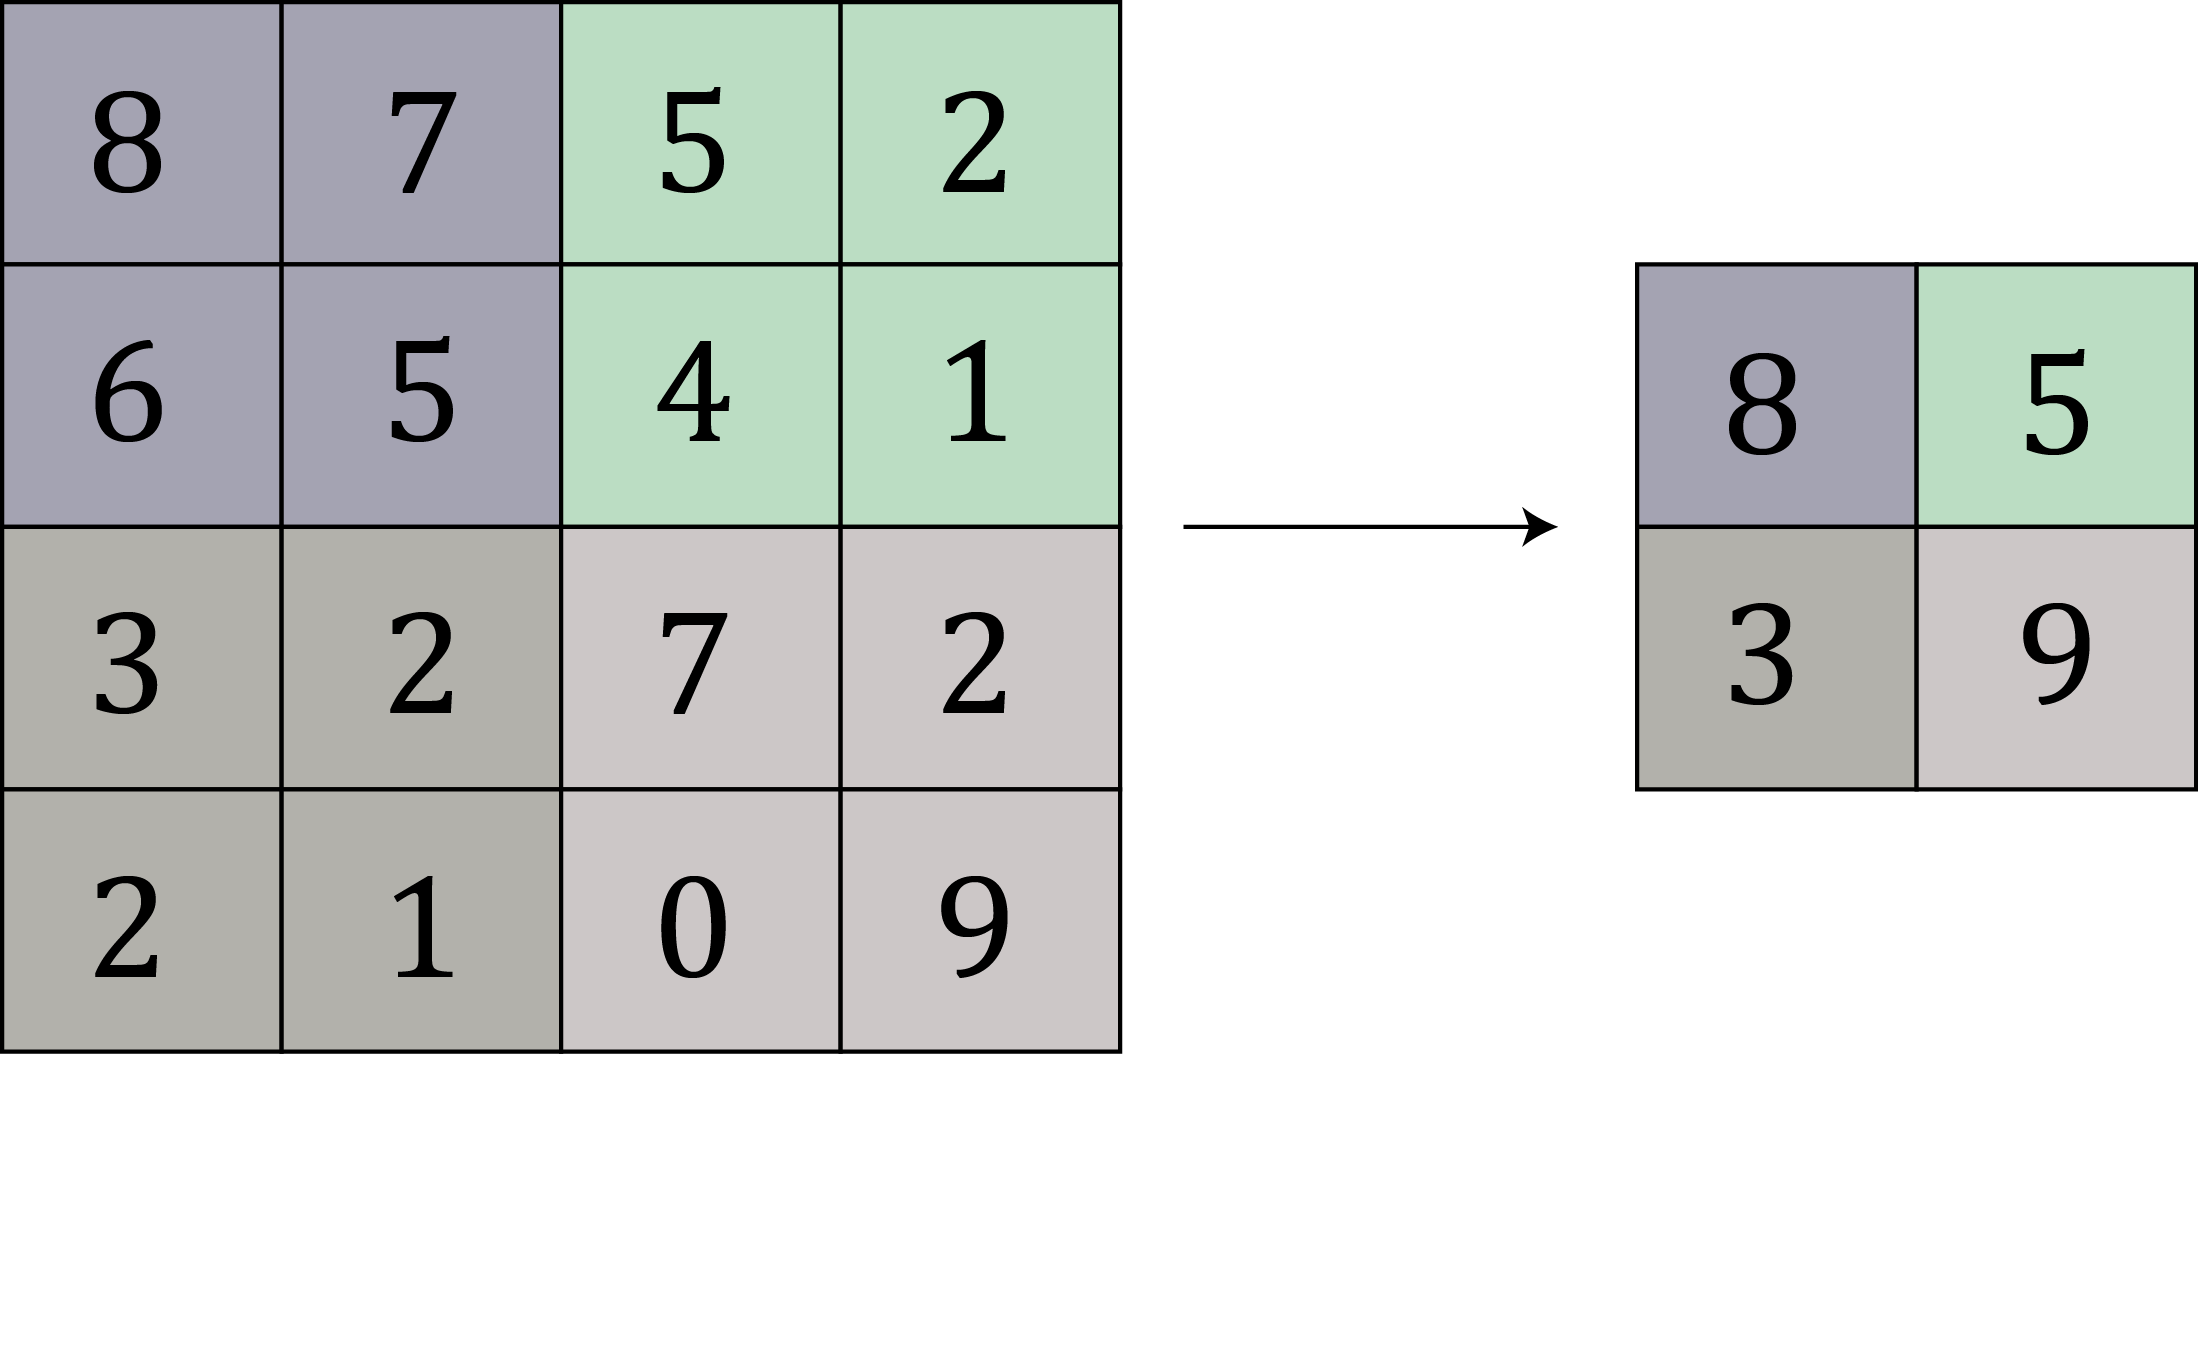
\includegraphics[width=8cm]{chaps/lr/max_pooling}}
	\caption{
		تابع \lr{max-pooling} بر روی آرایه دو بعدی کوچک $m=2$ و $s=2$
	}
	\label{fig:ch_lr:max_pooling}
\end{figure}
لایه کاملا متصل لایه آخر یک شبکه عصبی کانولوشنی محسوب می‌شود و اتصالات کاملی با خروجی لایه قبلی ایجاد می-کند. این لایه ورودی را دریافت و سپس خروجی را به صورت برداری با $N$ مولفه تولید می‌کند که $N$ تعداد کلاس‌هایی که شبکه باید طبقه بندی کند است. در واقع یک شبکه  \gls{convnet} جهت تولید یک بردار خروجی با $N$ مولفه عددی طراحی می‌شود که هر عدد در این بردار خروجی درصد احتمال تعلق به کلاس مورد نظر را نشان می‌دهد. برای یک مسئله با تعداد $k$  کلاس، $k$ نورون خروجی داریم که هر احتمال را با تابع \lr{SoftMax} محاسبه می‌کنند
\begin{equation}
	P(C)_j = \frac{e^{c_j}}{\sum^{K}_{k=1}e^{c_k}}
	\label{eq:ch_lr:softmax}
	%	\caption{محاسبه احتمال هر کلاس با تابع \lr{SoftMax}}
\end{equation}
اگر دو کلاس داشته باشیم می‌توانیم از تابع \lr{SoftMax} با دو خروجی استفاده کنیم یا از یک نورون استفاده کنیم و تابع \gls{sigmoid} را محاسبه کنیم. برای دو کلاس احتمال توسط معادله \ref{binary_softmax} محاسبه می‌شود
\begin{equation}
	P(1) = \frac{1}{1+e^i} \qquad \qquad P(0) = 1-P(1)
	\label{eq:ch_lr:binary_softmax}
	%	\caption{احتمال کلاس1 و احتمال کلاس0}
\end{equation}
\gls{dropout} یک روش بسیار رایج برای جلوگیری از \gls{overfitting} شبکه عصبی مصنوعی از جمله مدل‌های \gls{deeplearning} است\cite{srivastava2014dropout}.
ایده این تکنیک این است که با جلوگیری از هماهنگی نورون‌ها ، ویژگی‌های قوی تری ایجاد شود. اجرای آن ساده است تنها نیاز به بهم چسباندن لایه‌های اضافی در شبکه معمولا پس از توابع فعال سازی است. این ماژول بطور تصادفی برخی از نقاط نقشه ویژگی ورودی را  صفر می‌کند. هریک از ماژول‌ها دارای یک احتمال مستقل $\sigma$ برای نگهداری نقاط هستند و در صورت بروز چنین اتفاقی ، توسط  $\frac{1}{\sigma}$ مقیاس بندی می‌شوند. نقاطی که نگهداری نمی‌شوند بر روی صفر تنظیم می‌شوند. این لایه فقط یک پارامتر $\sigma$ دارد، که برای آموزش در فاصله $[0,1]$ قرار دارد و برای آزمایش روی $1$ قرار می‌گیرد. به طور شهودی، می‌توان این فرآیند را به عنوان حذف برخی از نورون‌های شبکه عصبی ، به طور موقت ، همراه با اتصالات ورودی و خروجی آن تصور کرد. مکانیزم حذف، نورون‌هایی را که به اتصالات ورودی کمتری متکی هستند را در نظرمی‌گیرد. زیرا افت یک زیر مجموعه از ورودی‌ها در مقایسه با یک نورون که به بسیاری از ورودی‌ها متکی است، قابل توجه‌تر خواهد بود و به این ترتیب ویژگی‌های کلی‌تر مهم‌تر می‌شوند. شکل \ref{fig:ch_lr:dropout} یک مثال از لایه \gls{dropout} را نمایش می‌دهد.
\begin{figure}[!ht]
	\centerline{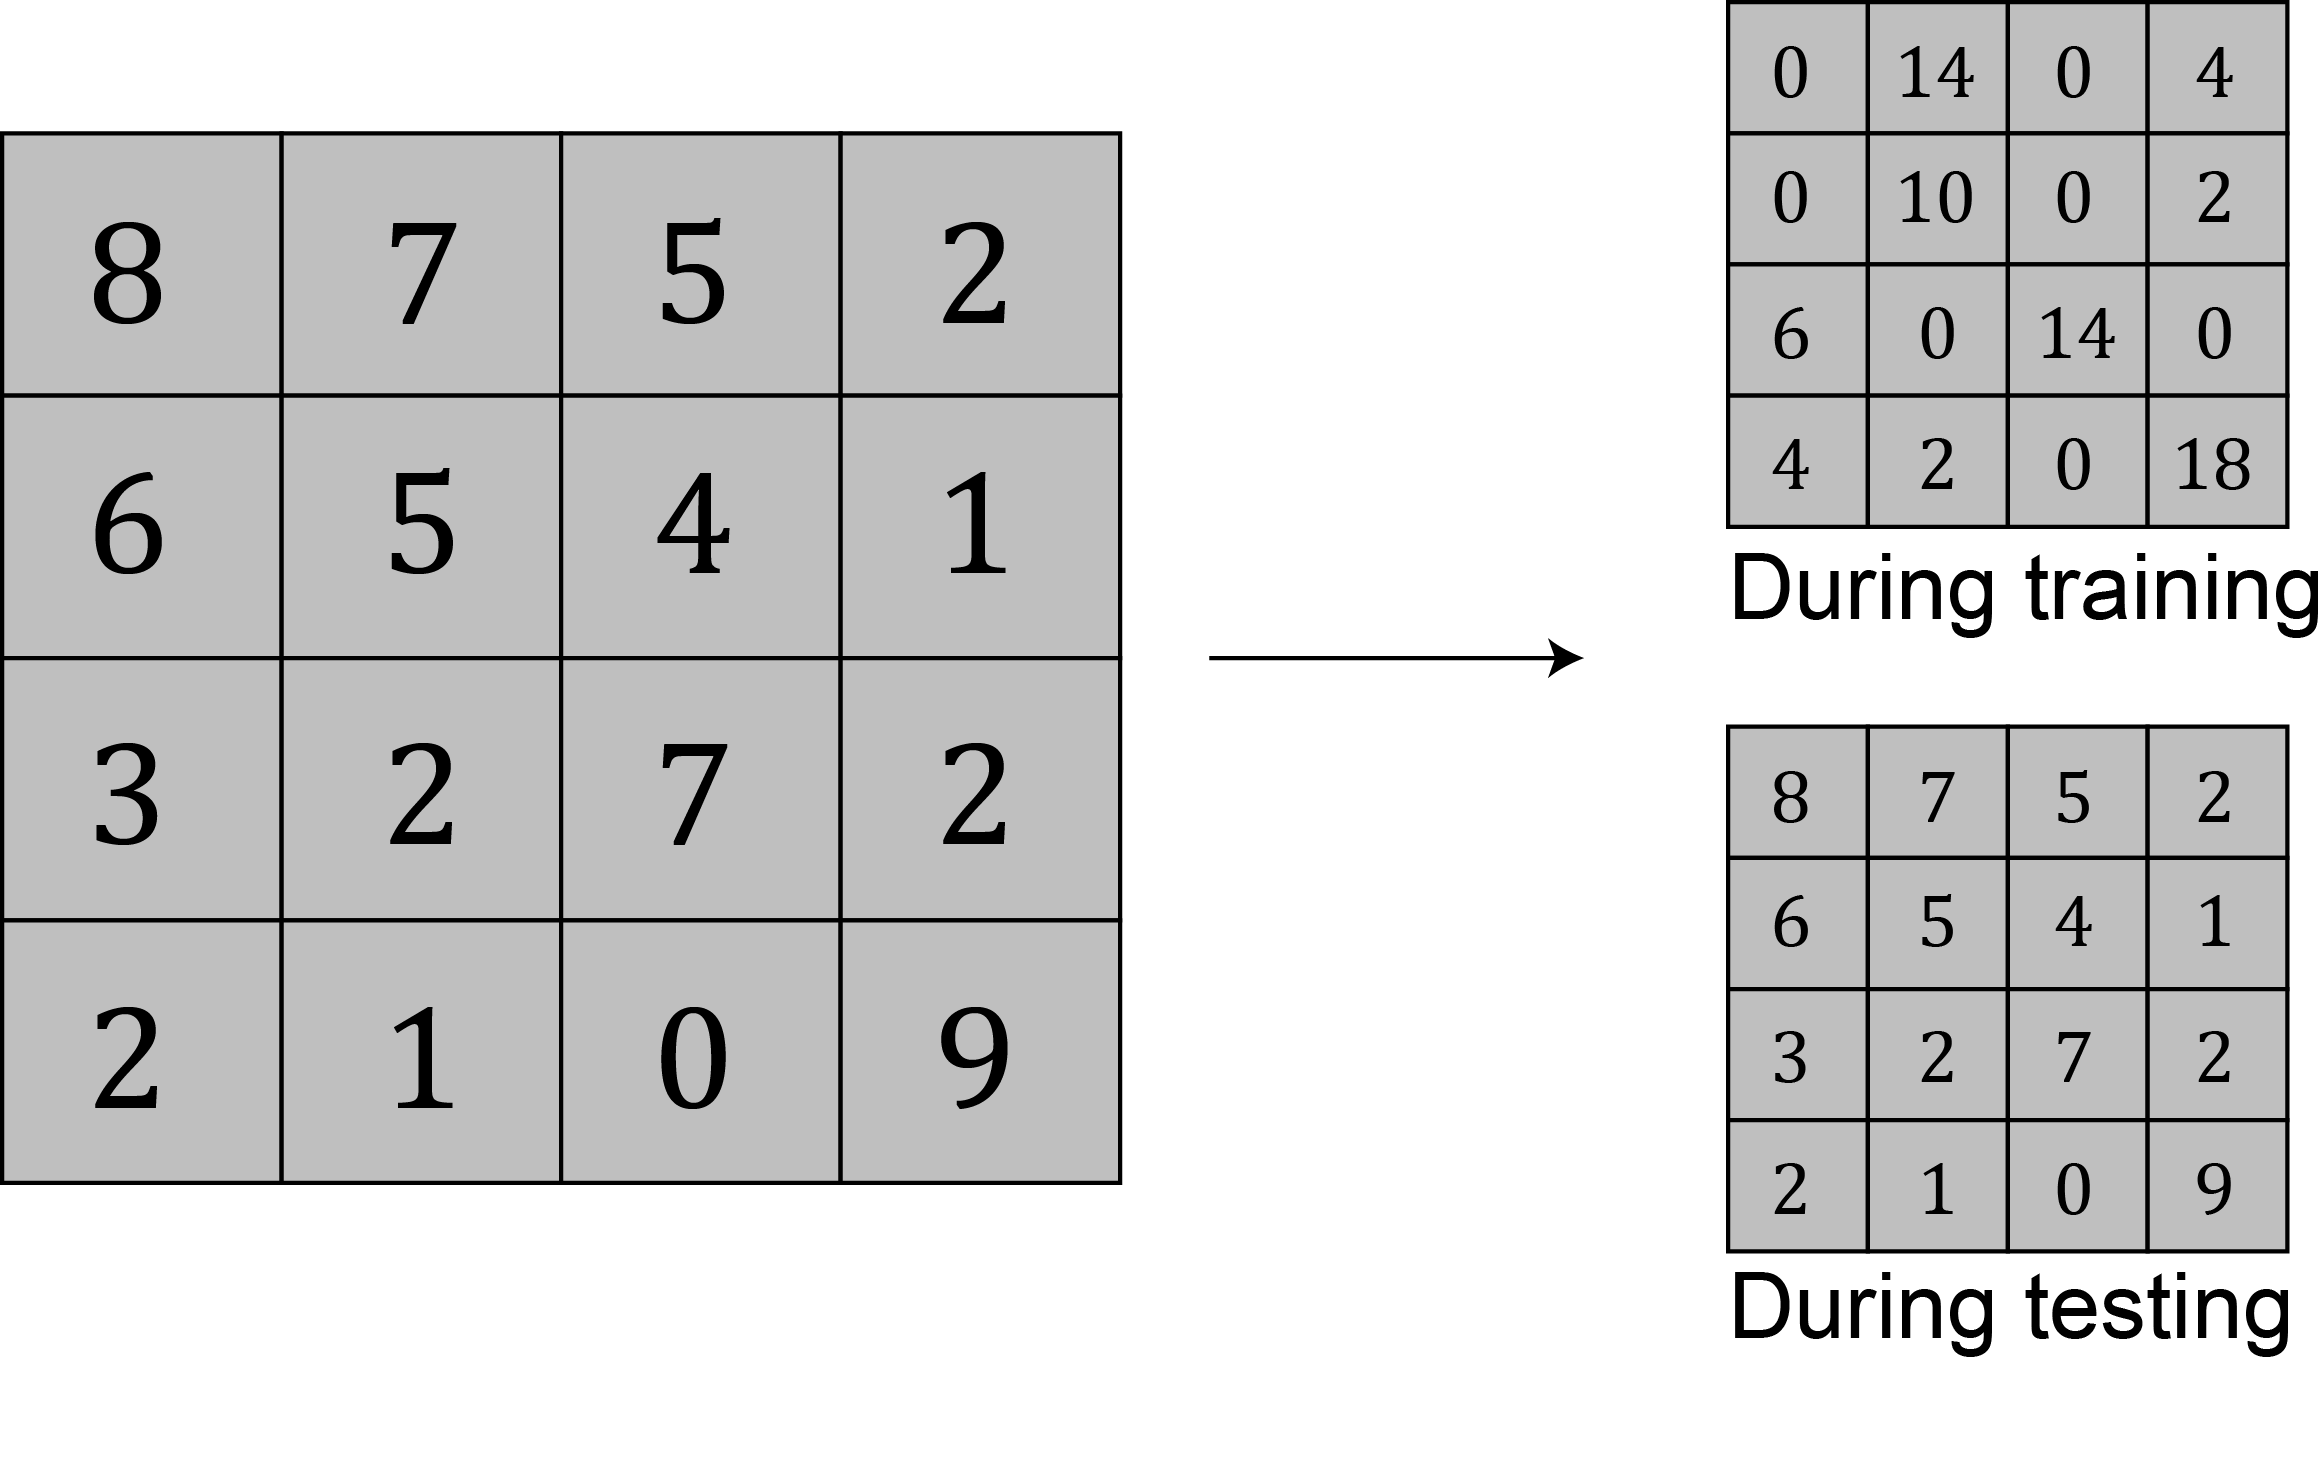
\includegraphics[width=10cm]{chaps/lr/dropout}}
	\caption{
		لایه \gls{dropout} با $\sigma=0.5$
	}
	\label{fig:ch_lr:dropout}
\end{figure}
\gls{batchnormalization} یک تکنیک جدید ولی خیلی کارامد است. در طی آموزش مدل‌های عمیق ، وزن‌ها در هر \gls{iteration}  به روز می‌شوند.
یک اثر جانبی این امر این است که در هر لایه توزیع‌های ورودی تغییر می‌کند، پدیده ای که به آن  \gls{internalcovariateshift}می‌گویند. این پدیده فرایند آموزش را کند می‌کند، به مقدار دهی دقیق‌تر وزن احتیاج دارد و مانع \gls{optimization} مدل‌های غیرخطی اشباع، مانند مماس‌های \gls{sigmoid} یا هایپربولیک می‌شود. برای حل این مشکل \gls{batchnormalization} را پیشنهاد می‌شود که مشابه با \gls{dropout}، به عنوان لایه ای در شبکه با رفتارهای متفاوت در حین آموزش و آزمون پیاده سازی می‌شود. برای رفع مشکل تغییر \gls{covariance} داخلی ، این لایه برای هر دسته آموزش  با کم کردن میانگین و تقسیم بر \gls{standarddeviation} همه نورون‌های عمق مشابه، ورودی خود را نرمال می‌کند. به میانگین و \gls{standarddeviation} آمار \lr{mini-batch}  گفته می‌شود. برای اطمینان از اینكه مدل می‌تواند دقیقاً همان تابع را با یا بدون \gls{batchnormalization} عادی نشان دهد ، دو وزن جدید قابل تمرین $\gamma$ و $\beta$ اضافه می‌شوند كه خروجی را اندازه گیری و جبران می‌كنند. بنابراین خروجی به صورت معادله \ref{eq:ch_lr:batch_normalization} است.
\begin{equation}
	\begin{aligned}
		\text{در طی آموزش}&: \quad I_c = \gamma \left(\frac{I_c-\text{\lr{mean}}(I_c)}{\text{\lr{std}}(I_c)}\right)+\beta  
		\\
		\text{در طی آزمایش}&: \quad I_c = \gamma \left(\frac{I_c-u_c}{v_c}\right)+\beta  
	\end{aligned}
	\label{eq:ch_lr:batch_normalization}
	%	\caption{احتمال کلاس1 و احتمال کلاس0}
\end{equation}
که $u_c$ و $v_c$ متوسط‌های در حال اجرا $\text{\lr{mean}}(I_c)$ و $\text{\lr{std}}(I_c)$ هستند. نشان داده شده است که \gls{batchnormalization} باعث آهنگ یادگیری بالاتر می‌شود و مدل در تکرارهای کمتری همگرا خواهد شد. این روش دارای اثر \gls{regularization} است. 
مدل با استفاده از \gls{costfunction} یاد می‌گیرد. این روشی است برای ارزیابی اینکه تا چه میزان خوب یک الگوریتم داده‌های مشاهده شده را می‌تواند مدل سازی کند. اگر پیش بینی‌ها بیش از حد از نتایج واقعی منحرف شوند ، \gls{costfunction} مقدار بالایی خواهد داشت. به تدریج، با کمک برخی توابع بهینه سازی، تابع هزینه می‌آموزد تا خطا در پیش بینی را کاهش دهد.

بهینه سازی مهمترین بخش در الگوریتم‌های یادگیری عمیق است. این کار با تعریف \gls{costfunction} شروع می‌شود و با به حداقل رساندن آن با استفاده از یک روش بهینه سازی به پایان می‌رسد. فرض کنید یک مجموعه داده $D$ با تعداد $I$ تصویر داریم. این تصاویر می‌توانند ضایعه باشند یا نباشند، بنابراین دارای برچسب $y\in \{0,1\}$ هستند.

باید مدلی بسازیم که با توجه به یک تصویر ورودی $I_i$، یک احتمال $p(I_i)$ تولید کند که تا حد ممکن به برچسب مربوط به آن تصویر ($y_i$) نزدیک باشد. برای این منظور الگوریتم‌های بهینه سازی متفاوتی وجو دارد مانند \lr{Adam}، \lr{SGD}\LTRfootnote{Stochastic gradient descent} و 
\lr{Adadelta}.\\
به حداقل رساندن \gls{costfunction} با کاهش گرادیان تقریباً رایج ترین الگوریتم برای بهینه سازی شبکه‌‌های عصبی است. اگر \gls{costfunction} \gls{binarycrossentropy} باشد و بخواهیم محاسبه کنیم که $p(I_i)$ تا چه حد خوب می‌تواند برچسب $y_i$ را تقریب بزند از معادله \ref{eq:ch_lr:binary_ce} استفاده می‌شود.
\begin{equation}
	L = \frac{1}{|\mathcal{D}|}  \sum_i^{|\mathcal{D}|}\Big(y_i \log\big(P(I_i)\big) + (1-y_i) \log\big(1-P(I_i)\big)\Big)
	\label{eq:ch_lr:binary_ce}
	%	\caption{تابع خطا cross-entropy binary}
\end{equation}
احتمال برای یک ورودی به وزن‌های آن ($\theta$) بستگی دارد و با
$p(I, \theta)$ 
نمایش داده می‌شود. با توجه به $\theta$ می‌توان $L(\theta)$ را با اجرای مدل بر روی مجموعه داده به دست آورد.

\gls{backpropagation}
اساس آموزش شبکه عصبی است. این عمل تنظیم-دقیق  وزن‌های یک شبکه عصبی بر اساس میزان \gls{loss} در هر \gls{epoch} قبلی است که این امر با محاسبه مشتق‌های تابع خطا بر اساس وزن‌ها 
$\nabla_\theta L(\theta)$
در زمان آموزش امکان پذیراست. تنظیم مناسب وزن‌ها  باعث کاهش میزان خطا می‌شود. در فرایند \gls{backpropagation}  ابتدا ورودی در سراسر شبکه انتشار داده می‌شود سپس $L(\theta)$ محاسبه شده و در نهایت این \gls{loss} از طریق تمام وزن‌ها در شبکه رو به عقب منتشر می‌شود. مشتق \gls{costfunction} از خروجی توسط معادله \ref{eq:ch_lr:dif_cf} محاسبه می‌شود.
\begin{equation}
	\frac{\partial L}{\partial P} = \frac{\partial \Big(-\big(y_i \log(p) + (1-y)\log(1-P)\big)\Big)}{\partial P} = \frac{P-y}{P(1-P)}
	\label{eq:ch_lr:dif_cf}
	%	\caption{محاسبه مشتق از تابع هزینه}
\end{equation}
همچنین محاسبه مشتق \gls{costfunction} $L$ از ورودی $i$ به صورت معادله \ref{eq:ch_lr:dif_cf_i} محاسبه می‌شود.
\begin{equation}
	\frac{\partial L}{\partial i} = \frac{\partial L}{\partial P} \frac{\partial P}{\partial i} = P-y
	\label{eq:ch_lr:dif_cf_i}
\end{equation}
همچنین محاسبه مشتق \gls{costfunction} بر اساس وزن‌های لایه آخر $w$ به صورت، 
\begin{equation}
	\frac{\partial L}{\partial w} = \frac{\partial L}{\partial P} \frac{\partial P}{\partial i}  \frac{\partial i}{\partial w}= (P-y)a
	\label{eq:ch_lr:dif_cf_w}
\end{equation}
می‌باشد که $a$ در آن برابر با ترکیب خطی از ورودی‌های لایه آخر است. این کار را می‌توان به راحتی به لایه‌های قبلی تعمیم داد، بنابراین می‌توان $\nabla _\theta L(\theta)$ را محاسبه کرد.